\documentclass[12pt]{article}

\usepackage[dvips,letterpaper,margin=0.75in,bottom=0.5in]{geometry}
\usepackage{cite}
\usepackage{slashed}
\usepackage{graphicx}
\usepackage{amsmath}
\usepackage{amssymb}
\usepackage{braket}
\usepackage{feynman}
\begin{document}

\newcounter{exercise}
\setcounter{exercise}{0}

\newcommand{\exercise}{
\stepcounter{exercise}
\noindent
{\bf Exercise \theexercise:}
}



\title{PHY 130A \\ Lecture Notes: \\ 
The Dirac Equation }
\author{Michael Mulhearn}

\maketitle

\section{The Four Gradient and Four-Momentum Operator}

In vector calculus, we define the gradient of a scalar-valued function $\phi(x,y,z)$ by:
$$\nabla \phi \;\equiv\; i \frac{\partial \phi}{\partial x} + j \frac{\partial \phi}{\partial y} + k \frac{\partial \phi}{\partial z} \;\equiv\; e_1 \frac{\partial \phi}{\partial x^1} + e_2 \frac{\partial \phi}{\partial x^2} + e_3 \frac{\partial \phi}{\partial x^3}$$
which we have written in two notations, so that you can see the components are simply:
$$\frac{\partial \phi}{\partial x^i}$$
Similarly, for a scalar valued function $f(x)$ of a four-vector $x$ with components $x^\mu$ we define the {\bf four-gradient} by its components:
$$\partial_\mu f \equiv \frac{\partial f}{\partial x^\mu}$$
In the exercise, you will show that $\partial_\mu f$ transforms like
the covariant components of a four vector, justifying our notation
(using lowered index) and establishing the four-gradient of a scalar
function as a four-vector.

Just as we write $\nabla$ as an operator without reference to a
specific function (as in $\nabla \phi$), we can likewise write:
$$\partial_\mu \equiv \frac{\partial}{\partial x^\mu}$$

\exercise (*) The components $x^\mu$ of the four-vector $x$  transform as:
$$ x^{\mu'} = \Lambda^{\mu '}_{\nu} x^{\nu}$$
and
$$ x^{\nu} = \Lambda^{\nu}_{\mu'} x^{\mu'}$$
For any scalar function
$f(x)$, show that the components $\partial_\mu f$ of the four-gradient
of $f$ transform as:
$$\partial_\mu f =  \Lambda_{\mu}^{\nu'} \partial_{\nu'} f$$
Hint:  Use the chain rule, and note that:
$$\frac{\partial x^\mu}{\partial x^{\nu'}} = \Lambda^{\mu}_{\nu'}$$
$\square$\\[5pt]

\exercise Let $\mathcal{B}$ be the standard basis for the four-vector space, so e.g.:
$$[x]_\mathcal{B} = \begin{pmatrix} x^0 \\ x^1 \\ x^2 \\ x^3 \end{pmatrix} $$
and $\mathcal{B}^*$ is as always the corresponding dual basis, so e.g.:
$$[x]_{\mathcal{B}^*} = \begin{pmatrix} x_0 \\ x_1 \\ x_2 \\ x_3 \end{pmatrix} $$
The covariant components $\partial_\mu$ of the
four-gradient, when written as a column vector in $\mathcal{B}^*$ are
$$[\partial]_{\mathcal \mathcal{B}^*} =
\begin{pmatrix}  \frac{\partial}{\partial t} \\[5pt]
\frac{\partial}{\partial x} \\[5pt]
\frac{\partial}{\partial y} \\[5pt]
\frac{\partial}{\partial z} \\
\end{pmatrix}
=
\begin{pmatrix}  \frac{\partial}{\partial t} \\[5pt]
\nabla \\[5pt]
\end{pmatrix}
$$
Show that the contravariant components $\partial^\mu$ of the
four-gradient, when written as a column vector in the standard basis
$\mathcal{B}$ are:
$$
[\partial]_{\mathcal B} =
\begin{pmatrix}  \frac{\partial}{\partial t} \\[5pt]
-\nabla \\[5pt]
\end{pmatrix}
$$
Hint: use the matrix representation of the metric tensor $G$.$\square$\\[5pt]

\exercise In Non-Relativistic Quantum Mechanics we replace the classical quantities total energy and momentum with operators:
$$E \to \hat{E} \equiv i\hbar \frac{\partial}{\partial t}, \hspace{2cm}
\vec{p} \to \hat{\vec{p}} \equiv -i\hbar \nabla
$$
Following this same prescription, show that the four-momentum operator is:
$$\hat{p}^\mu = i\hbar \partial^\mu$$
and
$$\hat{p}_\mu = i\hbar \partial_\mu$$

\section{Klein-Gordon Equation}
One approach to developing a relativistic quantum mechanics is
to start with the relativistic energy equation:
$$E^2 = p^2 + m^2$$
which can be written in terms of a four-vector squared as:
$$p^\mu p_\mu - m^2 = 0$$
And make the replacement:
$$p_\mu \to i \hbar \partial_\mu$$
The result is the Klein-Gordon equation:
$$-\hbar^2 \partial_\mu \partial^\mu \psi - m^2 \psi = 0$$
or equivalently:
$$-\frac{\partial^2 \psi}{\partial t^2} + \nabla^2 \psi = \left(\frac{m}{\hbar}\right)^2 \psi$$

\exercise Show that
$$\psi = A \sin\left(\frac{E t}{\hbar}\right) $$
is a solution to KG equation, provided $E = \pm m$.$\square$\\[5pt]

\exercise Show that $|\psi|^2$ for the previous exercise cannot
possibly represent a probability density, by sketching it as function of time.
$\square$\\[5pt]

The existence of negative energy solutions (as shown in the exercises)
is not a fatal problem (as we shall see).  The problem is that
$|\psi|^2$ integrated over all space is not conserved.\\[5pt]

\exercise Show that
$$\partial_\mu(\psi^* \partial^\mu \psi - \psi \partial^\mu \psi^*) = 0$$
$\square$\\[5pt]

\exercise When
$$\partial_\mu j^\mu = 0$$
we say that $j^\mu$ is a {\bf conserved-current}.  Show that for a conserved current $j^\mu$
then:
$$\frac{d}{dt} \int j^0 d^3 x = 0$$
or equivalently:
$$Q \equiv \int j^0 d^3 x$$
is a constant, which we call the conserved charge.  (Hint: assume the conserved current vanishes at infinity.)$\square$\\[5pt]

The exercises show that for:
$$\rho \equiv i (\psi^* \partial^\mu \psi - \psi \partial^\mu \psi^*)$$
we could normalize the wave function such that
$$\int \rho d^3x = 1$$
always.  However, we cannot interpret $\rho$ as a probability density
because it is not positive definite, as the next exercise will show.\\[5pt]

\exercise (*) Show that:
$$\psi = A \exp(-i E t / \hbar)$$
is a solution to the KG equation if $E = \pm m$, and in this case:
$\rho = 2E |\psi|^2$
which is less than zero for $E = -m$.$\square$\\[5pt]

This renders the K-G equation unsuitable for our current purposes of
finding a single particle wave function consistent with special
relativity.  However, in Quantum Field Theory, the notion of a single
particle with positive definite probability density is abandoned, and
the K-G equation emerges again as a perfectly valid equation for
describing spin-0 particles.

Historically, Schrodinger first derived the K-G equation, but
abandoned it when it failed to accurately predict the spectrum of the
Hydrogen atom.  This is because the electron in the Hydrogen atom is a
spin-1/2 particle, and is not described by the KG.  The (perceived)
shortcomings of the K-G equation arise from the fact that it is
quadratic in energy, which leads to a second order derivative in time.
And this led Dirac to seek an alternative approach.

\section{Dirac's Inspiration}

For what is coming next let's first consider the brave mathematicians who boldly asserted that one could take the square root of negative number, by assuming the existence of the imaginary unit $i$ with the defining property:
$$i^2 = -1$$
and carefully following that assertion through to all of its logical consequences.  They discovered the complex numbers, complex algebra, and brought us an indispensable new tool.  Imagine trying to do Quantum Mechanics without complex numbers!  The complex numbers also gave us profound new insights.  Something very similar is about to happen here!

The negative energy solutions to the Klein-Gordon equation result from
the square of the energy in the relativistic energy equation:
$$E^2 = p^2 + m^2$$
Non-relativistic Quantum Mechanics has no such difficulties because the energy equation is:
$$E = \frac{p^2}{2m}$$

Dirac considered the equation:
$$E = \sqrt{p^2 + m^2}$$
and thought that we must be able to replace $p$ with an operator and
still take that square root.  When he followed that through to its
logical conclusions, he discovered quantum field theory.  Our
approach, in the next section, will be based on factoring the
quadratic relativistic energy equation: So if Dirac's square root is
$\alpha$, we will be factoring:
$$0 = E^2 - \alpha^2 = (E-\alpha)(E+\alpha)$$

\section{Dirac Equation}
Following Dirac, we are attempting to factor the equation:
$$0 = p^\mu p_\mu - m^2 $$
by finding appropriate $\gamma^\mu$ and $\beta^\mu$ such that:
$$p^\mu p_\mu - m^2  = (\beta^\mu p_\mu + m) (\gamma^\omega p_\omega - m)$$
Calculating:
$$(\beta^\mu p_\mu + m) (\gamma^\omega p_\omega - m) 
= \beta^\mu \gamma^\omega p_\mu p_\omega - m^2 + m (\gamma^\omega p_\omega - \beta^\mu p_\mu)$$
When dealing with the last term, note that we are free to adjust the dummy indices so that:
$$\gamma^\omega p_\omega - \beta^\mu p_\mu = (\gamma^\mu - \beta^\mu) p_\mu$$
which amounts to combining terms with the same indices from two different sums.  We can therefore conclude that the unneeded and unwanted terms that are linear in $p^\mu$ can be eliminated simply by taking $\beta^\mu = \gamma^\mu$.  So we have now:
$$p^\mu p_\mu - m^2  = (\gamma^\mu p_\mu + m) (\gamma^\omega p_\omega - m)$$
which we will write out explicitly on both sides as:
\begin{multline*}
(p^0)^2-(p^1)^2-(p^2)^2-(p^3)^2-m^2 \\
= (\gamma^0)^2 (p^0)^2 + (\gamma^1)^2 (p^1)^2 + (\gamma^2)^2 (p^2)^2 + (\gamma^3)^2 (p^3)^2
-m^2 + {\rm CTs}
\end{multline*}
where we have neglected the cross-terms (CTs) and have used, for example, $(p_1)^2=(p^1)^2$.  We can match each term on LHS with one on the RHS if we arrange that:
\begin{equation}
\label{eqn:gammasq}
(\gamma^0)^2=1, \hspace{1cm} (\gamma^1)^2=-1,  \hspace{1cm} (\gamma^2)^2=-1,
 \hspace{1cm} (\gamma^3)^2=-1
\end{equation}
Then we will have equality as long as the cross-terms are all zero.  The cross terms are of form
$$\gamma^0 \gamma^1 p_0 p_1 + \gamma^1 \gamma^0 p_1 p_0$$
And now we have to face a bit of cold reality.  The terms $p_0$ and $p_1$ are coefficients of a four vector, just numbers, so they commute.  If $\gamma^0$ and $\gamma^1$ are simply coefficients, numbers, than they commute too, and so the cross terms simplify to quantities like:
$$2 \gamma^0 \gamma^1 p_0 p_1$$
Now as the cross-terms have to be zero for all possible $p^\mu$, we would need $\gamma^0 \gamma^1 = 0$, which would mean either $\gamma^0 = 0$ for $\gamma^1=0$.  But this is impossible to reconcile with the condition that $(\gamma^0)^2 = 1$ and $(\gamma^1)^2 = -1$.
But what if the $\gamma^\mu$ are matrices?  In this case, they need not commute, and the cross terms are of the form:
$$(\gamma^\mu \gamma^\omega + \gamma^\omega \gamma^\mu) p_\mu p_\omega$$
Notice that we have still commuted the $p_\mu$ and $p_\omega$ which are still the components of four-vectors, i.e. just numbers.  So we need matrices with the property that:
\begin{equation}
\label{eqn:gammacross}
\gamma^\mu \gamma^\omega + \gamma^\omega \gamma^\mu = 0, \hspace{1cm} (u \neq w)
\end{equation}
Using the {\bf anti-commutator} between $A$ and $B$ defined as:
$$\{A, B\} \equiv A B + B A$$
we can compactly express the requirements of Equations~\ref{eqn:gammasq} and \ref{eqn:gammacross} as:
\begin{equation}
\label{eqn:gammaanti}
\{\gamma^\mu, \gamma^\omega\} = \gamma^\mu \gamma^\omega + \gamma^\omega \gamma^\mu
= 2 g^{\mu \omega}
\end{equation}
This is the defining characteristic of the gamma group.  Any set of objects that satisfy the commutator relationship will do.  We will use the Dirac basis ($D$) in which these are 4x4 matrices of complex numbers:
$$[\gamma^0]_D = \begin{pmatrix} 
1 & 0 & 0 & 0 \\ 
0 & 1 & 0 & 0 \\ 
0 & 0 &-1 & 0 \\ 
0 & 0 & 0 &-1 \\ 
\end{pmatrix} \;\;
[\gamma^1]_D = \begin{pmatrix} 
0 & 0 & 0 & 1 \\ 
0 & 0 & 1 & 0 \\ 
0 &-1 & 0 & 0 \\ 
-1& 0 & 0 & 0 \\ 
\end{pmatrix} \;\;
$$
and:
$$
[\gamma^2]_D = \begin{pmatrix} 
 0 & 0 & 0 &-i \\ 
 0 & 0 & i & 0 \\ 
 0 & i & 0 & 0 \\ 
-i & 0 & 0 & 0 \\ 
\end{pmatrix} \;\;
[\gamma^3]_D = \begin{pmatrix} 
0 & 0 & 1 & 0 \\ 
0 & 0 & 0 &-1 \\ 
-1& 0 & 0 & 0 \\ 
0 & 1 & 0 & 0 \\ 
\end{pmatrix}.
$$
There are an infinite number of matrices that satisfy these
requirements but the smallest dimensions are 4x4 in dimension, as for
the Dirac basis.  When the choice of Dirac basis is clear, we will
often omit the $[\ldots]_D$, which is more conventional presentation
but less explicit.

There are more compact ways to write the gamma matrices, while still
remaining in the Dirac basis.
\begin{equation}
\label{eqn:gammamats}
[\gamma^0]_D = \begin{pmatrix} I & 0 \\ 0 & -I \end{pmatrix}, \hspace{2cm}
[\gamma^i]_D = \begin{pmatrix} 0 & \sigma^i \\ -\sigma^i & 0 \\ \end{pmatrix}
\hspace{1cm} (i=1,2,3)
\end{equation}
where $I$ is the 2x2 identity matrix:
$$I = \begin{pmatrix} 1 & 0 \\ 0 & 1 \end{pmatrix} $$
and the three $\sigma^i$ are the Pauli spin matrices:
$$\sigma^1 = \begin{pmatrix} 0 & 1 \\ 1 & 0 \end{pmatrix}, \hspace{2cm}
\sigma^2 = \begin{pmatrix} 0 & -i \\ i & 0 \end{pmatrix}, \hspace{2cm}
\sigma^3 = \begin{pmatrix} 1 & 0 \\ 0 & -1 \end{pmatrix}\\
\hspace{1cm} 
$$

With a solution in hand, we now return to our original problem, which was to factor the relativistic energy equation as:
$$p^\mu p_\mu-m^2 = \left( \gamma^\mu p_\mu - m \right) \left( \gamma^\omega p_\omega + m \right) = 0$$
Setting either of the two factors equal to zero will set the entire equation to zero (as needed).  It only makes a superficial difference which one we choose, but the conventional choice is to set:
$$\gamma^\mu p_\mu - m = 0$$
Now we can make the substitution:
$$p_\mu \to i \hbar \partial_\mu$$
To obtain the Dirac Equation:
\begin{equation}
\label{eqn:dirac}
i\hbar\gamma^\mu\partial_\mu \psi - m \psi = 0
\end{equation}
Notice that $\psi$ can not be a scalar function in the Dirac basis,
for that would have us adding a scalar to a 4x4 matrix.  The simplest
solution is for $\psi$ to be a four element column matrix:
$$[\psi]_D = \begin{pmatrix} \psi_1 \\ \psi_2 \\ \psi_3 \\ \psi_4 \\ \end{pmatrix}$$
Despite having four components, $\psi$ is {\bf not} a four-vector because (as we will show later) it does not transform like a four-vector.

\section{Solutions to the Dirac Equation}

We'll find solutions to the Dirac equation:
$$i\hbar \gamma^\mu \partial_\mu \psi -m \psi = 0$$
Let's first consider solutions with $\vec{p}=0$, so:
$$\frac{\partial\psi}{\partial x} = \frac{\partial\psi}{\partial y} = \frac{\partial\psi}{\partial z} = 0$$
and the Dirac equation becomes:
$$\gamma^0 \frac{\partial \psi}{\partial t} = -i \frac{m}{\hbar} \psi $$
Writing this out the long way in the Dirac representation:
$$
\begin{pmatrix} 
1 & 0 & 0 & 0\\
0 & 1 & 0 & 0\\
0 & 0 &-1 & 0\\
0 & 0 & 0 &-1\\
\end{pmatrix}
\frac{\partial}{\partial t}
\begin{pmatrix} 
\psi_1\\
\psi_2\\
\psi_3\\
\psi_4\\
\end{pmatrix}
=
-i \frac{m}{\hbar}
\begin{pmatrix} 
\psi_1\\
\psi_2\\
\psi_3\\
\psi_4\\
\end{pmatrix}
$$
or
$$
\frac{\partial}{\partial t}
\begin{pmatrix} 
\psi_1\\
\psi_2\\
-\psi_3\\
-\psi_4\\
\end{pmatrix}
=
-i \frac{m}{\hbar}
\begin{pmatrix} 
\psi_1\\
\psi_2\\
\psi_3\\
\psi_4\\
\end{pmatrix}
$$
There are four independent solutions:
$$
[\psi^{(1)}]_D = N \exp\left(- i \frac{m}{\hbar} t\right)
\begin{pmatrix} 
1\\
0\\
0\\
0\\
\end{pmatrix},
\hspace{1cm}
[\psi^{(2)}]_D = N \exp\left(- i \frac{m}{\hbar} t\right)
\begin{pmatrix} 
0\\
1\\
0\\
0\\
\end{pmatrix},
$$
and
$$
[\psi^{(3)}]_D = N \exp\left(+ i \frac{m}{\hbar} t\right)
\begin{pmatrix} 
0\\
0\\
1\\
0\\
\end{pmatrix},
\hspace{1cm}
[\psi^{(4)}]_D = N \exp\left(+ i \frac{m}{\hbar} t\right)
\begin{pmatrix} 
0\\
0\\
0\\
1\\
\end{pmatrix},
$$
where $N$ is a normalization factor.

Recalling that the energy operator is:
$$E = i\hbar \frac{\partial}{\partial t}$$
We see that:
$$ i\hbar \frac{\partial \Psi^{(1)}}{\partial t} = m \Psi^(1) \hspace{1cm}
i\hbar \frac{\partial \Psi^{(2)}}{\partial t} = m \Psi^{(2)}$$ 
and:
$$ i\hbar \frac{\partial \Psi^{(3)}}{\partial t} = -m \Psi^(3) \hspace{1cm}
i\hbar \frac{\partial \Psi^{(4)}}{\partial t} = -m \Psi^{(4)}$$ 
So evidently $\Psi^{(1)}$ and $\Psi^{(2)}$ have energy $E=m$ while $\Psi^{(3)}$
and $\Psi^{(4)}$ have energy $E=-m$.

I like to imagine Dirac laughing to himself at this point.  For
despite the great lengths he went through to develop a wave function
that is first order in Energy, we still arrive at negative energy
solutions.  And we cannot simply throw these solutions out on the
grounds that they are non-physical, because we would no longer have a
complete basis for our Hilbert space of bispinors.  As we'll see soon,
these negative energy solutions imply the existence antiparticles.
However, even setting aside the negative energy solutions for now,
that still leaves two solutions.  As we'll see later, this implies
that the Dirac equation applies to spin one-half particles (like the
electron), and the two positive energy solutions that we obtained are
for spin up and spin down states.

We should note that these solutions do not have the problem we
so readily encountered with solutions to the K-G equation. Specifically, for our solutions to a particle of mass $m$ at rest we see that:
$|\Psi|^2 = |N|^2 > 0$
independent of time for all four of these solutions.  More generally, it can be shown that
$$\frac{d}{dt}\int |\Psi(x,t)|^2 d^3x = 0$$
for all solutions to the Dirac equation, just as for the non-relativistic Schrodinger equation, and 
$|\Psi(x,t)|^2 \geq 0$.

\section{Antiparticles}


\begin{figure}[htbp]
\begin{center}

\begin{tabular}{cc}
  
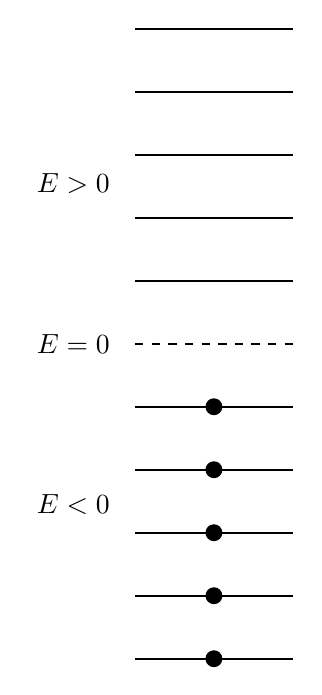
\begin{tikzpicture}[scale=1]

% Parameters
\def\levels{5}        % number of positive/negative levels
\def\ysep{0.8}        % vertical spacing between levels

% Draw positive energy levels (empty)
\foreach \i in {1,...,\levels} {
    \draw[thick] (-1.0,\i*\ysep) -- (1.0,\i*\ysep);
}

\draw[thick, dashed] (-1.0, 0) -- (1.0, 0);

% Draw negative energy levels (occupied with a single circle)
\foreach \i in {1,...,\levels} {
    \draw[thick] (-1.0,-\i*\ysep) -- (1.0,-\i*\ysep);
    \filldraw[black] (0,-\i*\ysep) circle (0.1);
}

% Labels
\node[left] at (-1.2,0) {$E=0$};
\node[left] at (-1.2,-2.3*\ysep-0.2) {$E<0$};
\node[left] at (-1.2,2.3*\ysep+0.2) {$E>0$};

\end{tikzpicture} & 

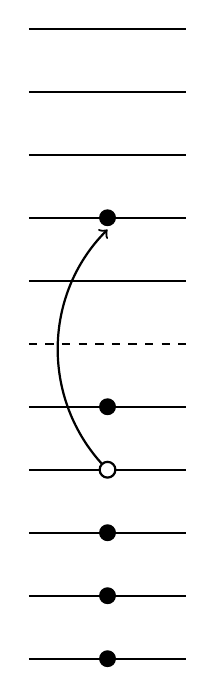
\begin{tikzpicture}[scale=1]

% Parameters
\def\levels{5}        % number of positive/negative levels
\def\ysep{0.8}        % vertical spacing between levels

% Draw positive energy levels (empty)
\foreach \i in {1,...,\levels} {
    \draw[thick] (-1.0,\i*\ysep) -- (1.0,\i*\ysep);
}

% Optional zero line (dashed)
\draw[thick, dashed] (-1.0, 0) -- (1.0, 0);

% Draw negative energy levels (occupied with a single circle)
\foreach \i in {1,...,\levels} {
    \draw[thick] (-1.0,-\i*\ysep) -- (1.0,-\i*\ysep);
    \filldraw[black] (0,-\i*\ysep) circle (0.1);
}

% Particle leaves negative energy state and appears in positive
\draw[->, thick, bend left=45] (0,-2*\ysep) to (0,2*\ysep-0.15);

% Indicate the hole in the negative sea
\filldraw[white] (0,-2*\ysep) circle (0.1);
\draw[thick] (0,-2*\ysep) circle (0.1); % outline of the hole

% Draw solid circle at new positive-energy location
\filldraw[black] (0,2*\ysep) circle (0.1);

\end{tikzpicture} \\
(a) & (b) \\
\end{tabular}
\caption{\label{fig:dirac-sea} In the vacuum (a) the negative energy
  states are all filled, forming the Dirac Sea.  A particle in a
  negative energy state can gain energy, occupying a positive energy
  state to produce a particle, and leaving behind a vacancy (or hole)
  in the Dirac sea, which is interpreted as an antiparticle.  }
\end{center}
\end{figure}

\noindent
Dirac postulated that the negative energy solutions represented actual
physical states.  To reconcile the existence of these states with
physical reality, he postulated that in the vacuum, the negative energy
states are all occupied, as shown in Fig.~\ref{fig:dirac-sea}.  The
Fermi exclusion principle then prevents ordinary particles from
falling down into the negative energy states, releasing an unlimited
amount of energy.

In this scenario, adding sufficient energy to a particle in a negative
energy state, will raise it to a positive energy state, and so create
an ordinary particle.  In so doing, it will leave behind a vacancy in
the Dirac sea.  The vacancy would behave as if a particle with
opposite charge to the ordinary particle had been created ($0 = q +
(-q)$).  This is a very workable (if implausible) description for the
creation of particle antiparticle pairs, and indeed it was sufficient
to predict the existence and properties of the positron, which was
later discovered by Anderson.

\begin{figure}[htbp]
\begin{center}
\begin{feynman}
    \fermion{0.5, 0.5}{0.0, 0.0}
    \fermion{0.0, 1.0}{0.5, 0.5}
    \electroweak{0.5, 0.5}{1.2, 0.5}
    \node at (-0.1,0.0) {$e$};
    \node at (-0.1,1.0) {$e$};
    \node at (1.3,0.5) {$\gamma$};
 \end{feynman}
\caption{\label{fig:fs-interpretation}  This Feynman diagram has three equivalent interpretations:  (1) two incident electrons, one with positive and one with negative energy, (2) two incident electrons, one propagating forward in time, and one propagating backward, (3) an incident electron and positron.}
\end{center}
\end{figure}

The energy eigenstates of particles with $E > 0$ have time-dependence:
$$\exp(-iEt/\hbar) = \exp(-i|E|t/\hbar) $$
whereas particles with $E < 0$ have time-dependence:
$$\exp(-iEt/\hbar) = \exp(+i|E|t/\hbar) $$ This suggests that
particles with negative energy can be reinterpreted as particles with
positive energy that propagate backwards in time.  We derived the
Dirac equation to be consistent with special relativity, and we have
already seen that time-reversal is a member of the Lorentz group.

This is best visualized in the context of a Feynman diagram, as in
Fig.~\ref{fig:fs-interpretation} In the Feynman-Stuckelberg
interpretation, particle states propagating backwards in time are
interpreted as antiparticle states propagating forward in time.
Whereas an incident particle of charge $q$ propagating forward in time
brings a charge $q$, an incident particle of charge $q$ propagating
backward in time carries away a charge $q$.  Thus we expect
antiparticles to carry the opposite charge of the corresponding
particle.  The energy of both particle and antiparticle is positive,
so the mass of the antiparticle does not change sign, and we expect
both particle and antiparticle to have the same positive mass.

Particles wave functions have time-dependence:
$$\exp(-iEt/\hbar)$$
and antiparticles wave functions have time dependence:
$$\exp(iEt/\hbar)$$
where $E>0$ in both cases is the physical energy of the particle.
Particles have momentum operator given by:
$$p_\mu = i \hbar \partial_\mu$$
which leads to:
$$p^0 = E$$
as expected.  Antiparticles must therefore have:
$$p_\mu = -i \hbar \partial_\mu$$
which leads to:
$$p^0 = E$$ as expected.  The angular momentum operator, through its
dependence on momentum, will also change sign.  Spin also changes
sign, otherwise, we could distinguish a particle with intrinsic spin
one from a composite system with total angular-momentum one.


\section{Notation}

There is some new notation to help us navigate the strange new world
Dirac revealed by taking his square-root.  Because the three Pauli
matrices ($\sigma^1, \sigma^2, \sigma^3$) are often associated with
the three spatial coordinates ($x, y, z$) we can consider them as a
forming a sort of three-vector:
$$\vec{\sigma} \; \equiv \; \sigma^1 \, \hat{x} + \sigma^2 \, \hat{y} + \sigma^3 \, \hat{z}$$
whose components are matrices instead of scalars.  This three-vector can be dotted with other three vectors, e.g.:
$$\vec{a} \cdot \vec{\sigma} = a_x \sigma^1 + a_y \sigma^2 + a_z \sigma^3
= \begin{pmatrix} a_z & a_x - i a_y \\ a_x + i a_y & -a_z \end{pmatrix}
$$
It is useful to note that:
\begin{eqnarray*}
(\vec{a} \cdot \vec{\sigma})^2 &=& (a_x \sigma^1 + a_y \sigma^2 + a_z \sigma^3)^2\\[5pt]
&=& a_x^2 (\sigma^1)^2 + a_y^2 (\sigma^2)^2 + a_z^2 (\sigma^3)^2 + {\rm CTs}\\
\end{eqnarray*}
The cross-terms (CTs) are all zero, as the Pauli matrices anti-commute, for example:
$$a_x a_y (\sigma^1 \sigma^2 + \sigma^2 \sigma^1) = 0$$
Recalling that also:
$$(\sigma^1)^2 = (\sigma^2)^2 = (\sigma^3)^2 = 1$$
we conclude:
$$(\vec{a}\cdot\vec{\sigma})^2 = |\vec{a}|^2$$

We encounter gamma matrices contracted with four vectors so often the combinations gets its own notation, the Feynman slash notation:
\begin{eqnarray*}
\slashed{a} &\equiv& \gamma^\mu a_\mu = a^0 \begin{pmatrix} I & 0 \\ 0 & -I \end{pmatrix}
- \vec{a} \cdot \begin{pmatrix} 0 & \vec{\sigma} \\ -\vec{\sigma} & 0 \end{pmatrix}\\
&=& \begin{pmatrix} a^0 I & - \vec{a}\cdot\vec{\sigma} \\ \vec{a}\cdot\vec{\sigma} & -a^0 I \end{pmatrix}
\end{eqnarray*}
While we are discussing notation, we won't be writing out $I$ explicitly much longer, when it can be inferred from context.  The above, for example, would usually be written as:
\begin{eqnarray*}
\slashed{a} &\equiv& \gamma^\mu a_\mu = a^0 \begin{pmatrix} 1 & 0 \\ 0 & -1 \end{pmatrix}
- \vec{a} \cdot \begin{pmatrix} 0 & \vec{\sigma} \\ -\vec{\sigma} & 0\end{pmatrix}\\
&=& \begin{pmatrix} a^0 & - \vec{a}\cdot\vec{\sigma} \\ \vec{a}\cdot\vec{\sigma} & -a^0 \end{pmatrix}
\end{eqnarray*}

\section{Plane Wave Solutions for Particles}

We are now ready to tackle the plane wave solutions.  You may recall
from NRQM that these are all we will need for describing scattering
experiments, since our experiments measure particles only far away
from the interaction potentials, at infinity effectively, where they
are free particles well described by plane waves (or a wave packet
from the superposition of plane waves).

We will therefore attempt to find particle solutions of the form:
$$\psi = a \, e^{-ikx} \, u(k)$$
where $a$ is a normalization factor, and the exponential contains a factor
$$kx = k^\mu x_\mu$$
which is the only space and time dependence.  The $u(k)$ is the bi-spinor part which we can write as either two spinors or four components:
$$[u(k)]_D \equiv \begin{pmatrix} u_A \\ u_B \\ \end{pmatrix} \equiv 
\begin{pmatrix} u_1 \\ u_2\\ u_3 \\ u_4 \end{pmatrix}
$$
The components are still dependent on $k$ but we have dropped the explicit dependence for brevity.

Note that:
$$\partial_\mu \psi = \frac{\partial \psi}{\partial x^\mu} = a \left( \frac{\partial}{\partial x^\mu} \exp(-ik_\mu x^\mu)\right) u(k) = -ik_\mu \psi$$
The Dirac equation:
$$i\hbar \gamma^\mu \partial_\mu \psi - m \psi = 0$$
when applied to the plane wave yields:
\begin{eqnarray*}
(\hbar \gamma^\mu k_\mu - m) \; \psi &=& 0 \\[5pt]
(\hbar \gamma^\mu k_\mu - m) \; a \, e^{-ikx} \, u(k) &=& 0 \\[5pt]
(\hbar \slashed{k} - m) \; u(k) &=& 0 \\[5pt]
\begin{pmatrix}
\hbar k^0-m & - \hbar \vec{k}\cdot\vec{\sigma} \\
\hbar \vec{k}\cdot\vec{\sigma} & -\hbar k^0-m \\
\end{pmatrix}
\begin{pmatrix} 
u_A\\
u_B\\
\end{pmatrix}&=&0\\
\end{eqnarray*}
Solving the last matrix equation we obtain:
\begin{eqnarray}
u_A &=& \frac{\hbar\vec{k}\cdot\vec{\sigma}}{\hbar k^0-m} u_B \label{eqn:ua} \\
u_B &=& \frac{\hbar\vec{k}\cdot\vec{\sigma}}{\hbar k^0+m} u_A \label{eqn:ub} \\
\notag
\end{eqnarray}
Plugging the second equation into the first:
\begin{eqnarray*}
u_A &=& \frac{(\hbar\vec{k}\cdot\vec{\sigma})^2}{(\hbar k^0)^2-(m)^2} u_A \\
    &=& \frac{\hbar^2|\vec{k}|^2}{(\hbar k^0)^2-(m)^2} u_A \\
(m)^2 &=& \hbar^2((k^0)^2-|\vec{k}|^2) = \hbar^2 k^\mu k_\mu \\
\end{eqnarray*}
But we already know a four-vector whose square is $m^2$, the four-momentum:
$$p^2 = (m)^2$$
We conclude that $p^\mu = \pm \hbar k^\mu$.  However, only $p^\mu = \hbar k^\mu$
leads to the correct time-dependence 
$$\psi = a \, e^{-ikx} \, u(k) = a \, \exp(- iEt/\hbar) \exp(i\vec{p}\cdot\vec{x}) u(k)$$
for a particle of energy $E$ and momentum $\vec{p}$.  We may rewrite Equation~\ref{eqn:ub} as:
$$u_B = \frac{\vec{p}\cdot\vec{\sigma}}{p^0+m} u_A = \frac{1}{E+m} \; \vec{p}\cdot\vec{\sigma} \; u_A$$
and writing out $\vec{p}\cdot\vec{\sigma}$ as a matrix:
$$u_B = \frac{1}{E+m} \; \begin{pmatrix} p_z & p_x - i p_y \\ p_x + i p_y & -p_z \\ \end{pmatrix} u_A
$$
And next we find two solutions by applying this result to a starting choice for $u_A$:
\begin{eqnarray*}
u_A = \begin{pmatrix} 1 \\ 0 \\ \end{pmatrix} &\implies& 
u_B = \frac{1}{E+m} \begin{pmatrix} p_z \\ p_x + i p_y \\ \end{pmatrix}\\
u_A = \begin{pmatrix} 0 \\ 1 \\ \end{pmatrix} &\implies& 
u_B = \frac{1}{E+m} \begin{pmatrix} p_x - i p_y \\ -p_z \\ \end{pmatrix}\\
\end{eqnarray*}
For particles, we can go no further.  If we attempt to make a choice for $u_B$, then we would be obliged to use Equation~\ref{eqn:ua}, which will blow up when $E=m$ due to the negative sign in the denominator.

We assemble $u_A$ and $u_B$ to form the entire bi-spinor for the particle solutions:
$$
[u^{(1)}]_D = N \begin{pmatrix} 1 \\ 0 \\ \frac{p_z}{E+m} \\[5pt] \frac{p_x + i p_y}{E + m} \end{pmatrix}, 
\hspace{1cm}
[u^{(2)}]_D = N \begin{pmatrix} 0 \\ 1 \\ \frac{p_x - i c p_y}{E+m} \\ \frac{-p_z}{E+m} \end{pmatrix}.
$$
where $N$ is a not-yet-determined normalization factor. \\[5pt]


\section{Plane Wave Solutions for Antiparticles}

Next we attempt to find antiparticle solutions of the form:
$$\psi = a \, e^{ikx} \, v(k)$$
where $a$ is a normalization factor, and the exponential contains a factor
$$kx = k^\mu x_\mu$$
which is the only space and time dependence.  The $v(k)$ is the bi-spinor part which we can write as either two spinors or four components:
$$[v(k)]_D \equiv \begin{pmatrix} v_A \\ v_B \\ \end{pmatrix} \equiv 
\begin{pmatrix} v_1 \\ v_2\\ v_3 \\ v_4 \end{pmatrix}
$$
In this case the Dirac equation
$$i\hbar \gamma^\mu \partial_\mu \psi - m \psi = 0$$
when applied to the plane wave yields:
\begin{eqnarray*}
(-\hbar \gamma^\mu k_\mu - m) \; a \, e^{ikx} \, v(k) &=& 0 \\[5pt]
(\hbar \slashed{k} + m) \; v(k) &=& 0 \\[5pt]
\begin{pmatrix}
\hbar k^0+m & - \hbar \vec{k}\cdot\vec{\sigma} \\
\hbar \vec{k}\cdot\vec{\sigma} & -\hbar k^0+m \\
\end{pmatrix}
\begin{pmatrix} 
v_A\\
v_B\\
\end{pmatrix}&=&0\\
\end{eqnarray*}
Solving the first row of matrix equation we obtain:
\begin{eqnarray}
v_A &=& \frac{\hbar\vec{k}\cdot\vec{\sigma}}{\hbar k^0+m} v_B \label{eqn:va} \\
%v_B &=& \frac{\hbar\vec{k}\cdot\vec{\sigma}}{\hbar k^0-m} v_A \label{eqn:vb} \\
\notag
\end{eqnarray}
By a similar calculation as in the previous section we conclude that:
$p^\mu = \pm \hbar k^\mu$.  However, only $p^\mu = \hbar k^\mu$
leads to the correct time-dependence 
$$\psi = a \, e^{ikx} \, v(k) = a \, \exp(iEt/\hbar) \exp(-i\vec{p}\cdot\vec{x}) v(k)$$
for an antiparticle of energy $E$ and momentum $\vec{p}$.  We may rewrite Equation~\ref{eqn:va} as:
$$v_A = \frac{\vec{p}\cdot\vec{\sigma}}{p^0+m} v_B = \frac{1}{E+m} \; \vec{p}\cdot\vec{\sigma} \; v_B$$
and writing out $\vec{p}\cdot\vec{\sigma}$ as a matrix:
$$v_A = \frac{1}{E+m} \; \begin{pmatrix} p_z & p_x - i p_y \\ p_x + i p_y & -p_z \\ \end{pmatrix} v_B
$$
And next we find two solutions by applying this result to a starting choice for $v_B$:
\begin{eqnarray*}
v_B = \begin{pmatrix} 1 \\ 0 \\ \end{pmatrix} &\implies& 
v_A = \frac{1}{E+m} \begin{pmatrix} p_z \\ p_x + i p_y \\ \end{pmatrix}\\
v_B = \begin{pmatrix} 0 \\ 1 \\ \end{pmatrix} &\implies& 
v_A = \frac{1}{E+m} \begin{pmatrix} p_x - i p_y \\ -p_z \\ \end{pmatrix}\\
\end{eqnarray*}
We assemble $v_A$ and $v_B$ to form the entire bi-spinor for the antiparticle solutions:
$$
[v^{(1)}]_D = N \begin{pmatrix} \frac{p_x - i p_y}{E+m} \\ \frac{-p_z}{E+m} \\ 0 \\ 1\end{pmatrix}.
\hspace{1cm}
[v^{(2)}]_D = -N \begin{pmatrix} \frac{p_z}{E+m} \\[5pt] \frac{p_x + i p_y}{E + m} \\ 1 \\ 0\end{pmatrix},
$$
The rationale for ordering the solutions this way, and the reason for the overall negative sign in front of $v^{(2)}$ will become clear in the exercises (e.g. Griffiths P7.9).

We will use $u$ for particles and $v$ for antiparticles.  The Dirac equation for particles in terms of the momentum now reads:
$$(\slashed{p}-m) u = 0$$
For antiparticles, $k^\mu = -p^\mu / \hbar$, and the Dirac equation reads:
$$(\slashed{p}+m) v = 0$$


\section{Review: Angular Momentum in Quantum Mechanics}

This section follows Griffith's Introduction to Quantum Mechanics,
Section 4.3, so you should refer to that if you get stuck on any of
the exercises.

The classical angular momentum is:
$$\vec{L} = \vec{r} \times \vec{p}$$
from which we determine the corresponding angular momentum operators using the position and momentum operators:
$$L_x \equiv y p_z - z p_y, \hspace{1cm} L_y \equiv z p_x - x p_z, \hspace{1cm} L_z \equiv x p_y - y p_x$$
and the total momentum squared:
$$L^2 = L_x^2 + L_y^2 +L_z^2$$
In the exercises, you will very that:
\begin{equation}
\label{eqn:lcom}
      [L_x,L_y] = i\hbar Lz, \hspace{1cm} [L_y,L_z] = i\hbar Lx, \hspace{1cm} [L_z,L_x] = i\hbar Ly
\end{equation}      
and
\begin{equation}
\label{eqn:lsqcom}
      [L^2,L_x] = [L^2,L_y] = [L^2,L_z] = 0
\end{equation}      
This shows that while $L_x$, $L_y$, and $L_z$ are incompatible
observables, $L^2$ commutes with any single component.  So we can
therefore find eigenstates of both $L^2$ and $L_z$.

Equation~\ref{eqn:lcom} reveals that there is a closed algebra of
commutators over the angular momentum operators.  We use an algebraic
approach based on the ladder operators:
$$L_{\pm} \equiv L_x + i L_y$$
for which you will show:
\begin{equation}
\label{eqn:lsqlpmcom}  
     [L^2,L_{\pm}] = 0
\end{equation}
and:
\begin{equation}
\label{eqn:lzlpmcom}  
     [L^2,L_{\pm}] = \pm \hbar L_{\pm}
\end{equation}
and:
\begin{equation}
\label{eqn:ltop}  
     L^2 = L_{\pm} L_{\mp} - L_z^2 \mp \hbar L_z
\end{equation}


\exercise Prove Equations~\ref{eqn:lcom}.  You need only prove it for one, then the rest follow from the cyclic rotation $xyz \to yzx$ which leaves the definitions unchanged.\\[5pt]

\exercise Prove Equations~\ref{eqn:lsqcom} You need only prove it for one, then the rest follow from the cyclic rotation $xyz \to yzx$.\\[5pt]

\exercise Prove Equations~\ref{eqn:lsqlpmcom}\\[5pt]

\exercise Prove Equation~\ref{eqn:lzlpmcom}\\[5pt]

\exercise Prove Equation~\ref{eqn:ltop}\\[5pt]

With the heavy lifting behind us, we can consider a simultaneous eigenstate of both $L^2$ and $L_z$ so that:
$$L^2 f = \alpha f$$
and 
$$L_z f = \mu f$$
Consider the state $L_+ f$. Using Equation~\ref{eqn:lsqlpmcom} we see that:
$$L^2 (L_+ f) = L_+ (L^2 f) = L_+ (\lambda f) = \lambda (L_+ f) $$
and using Equation~\ref{eqn:lzlpmcom} we see that:
$$L_z (L_+ f) = (L_+ L_z + \hbar L_+) f = (\mu + \hbar) (L_+ f) $$
This shows that $L_+ f$ remains an eigenstate of $L^2$ with the same eigenvalue as $f$, and also remains an eigenstate of $L_z$ but with new eigenvalue $\mu + \hbar$.  We say that $L_+$ is a raising operator.

We cannot keep applying the raising operator indefinitely, for eventually the square of the $z$ component of angular momentum would be larger than the $L^2$.  Therefore, after some number of applications of $L^+$ we must eventually reach a state $g$ for which:
$$L_+ g = 0$$
For convenience in what follows, let's define a dimensionless quantity $\ell$ by the eigenvalue of this ``top-rung'' state $g$:
$$L_+ g \equiv \ell \hbar g$$
In the exercises, you will show that:
$$L^2 g = \hbar^2 \ell (\ell+1) g$$
which relates the eigenvalue of $L^2$ (which we do not change via the raising operator) to the maximum eigenvalue of the $L_z$.

In a similar fashion, we see that the operator $L_-$ is a lowering
operator, so that $L_-f$ remains an eigenstate of $L^2$ with same
eigenvalue, and also remains an eigenstate of $L_z$ but with new
eigenvalue $\mu - \hbar$.  Also similarly, we cannot endlessly apply
$L_-$.  After some number of applications of $L_-$ we must reach a
state $h$ for which:
$$L_- h = 0$$
Again for convenience, we define a dimensionless quantity $\bar{\ell}$ by the eigenvalue of the ``bottom-rung'' state $h$:
$$L_z h \equiv \bar{\ell} \hbar h$$
In the exercises you will show that
$$L^2 h = \hbar^2 \bar{\ell} (\bar{\ell}-1) h$$

\exercise Using equation ~\ref{eqn:ltop} show that:
$$L^2 g = \hbar^2 \ell (\ell+1) g$$
and
$$L^2 h = \hbar^2 \bar{\ell} (\bar{\ell}-1) h$$
$\square$\\[5pt]

Comparing these results for the lower-rung with those of the upper rung, and noting that the raising operator leaves the the eigenvalue of $L^2$ unchanged, we conclude that 
$\ell(\ell+1) = \bar{\ell}(\bar{\ell}-1)$
So either
$$\bar{\ell} = \ell+1$$
which is impossible, since we must have the lower bound below the upper bound:
$$\bar{\ell}\hbar < \ell \hbar$$
or
$$\bar{\ell} = -\ell$$
This implies that $\ell$ is non-negative.  Furthermore, we move from $-\ell$ to $\ell$ in an integer number of applications of $N$, so:
$$-\ell + N = \ell$$
which implies that $\ell$ is integer or half-integer:
$$\ell = \frac{N}{2}$$

To summarize, the eigenstates $\ket{lm}$ of $L^2$ are $L_z$ are characterized by two quantum numbers:
$$\ell = 0, \frac{1}{2}, 1, \frac{3}{2}, 2, \ldots$$
and
$$m = -\ell, -\ell+1, \dots \ell$$
with:
$$L^2 \ket{lm} = \hbar^2 \ell (\ell+1) \ket{lm}$$
and
$$L_z \ket{lm} = \hbar m \ket{lm}$$

In the last exercise of this section, you will show that:
$$L_+ \ket{l\,m} = \hbar \sqrt{(l-m)(l+m+1)} \ket{l\,(m+1)}$$
Similarly:
$$L_- \ket{l\,m} = \hbar \sqrt{(l+m)(l-m+1)} \ket{l\,(m-1)}$$

\exercise Show that:
$$L_+ \ket{l\,m} = \hbar \sqrt{(l-m)(l+m+1)} \ket{l\,(m+1)}$$
Hint:  First put:
$$L_+ \ket{l\,m} = \alpha \ket{l\,m}$$
where $\alpha$ is the quantity we seek to calculate.  Notice that $L_+^\dagger = L_-$ and so:
$$\braket{l\,m|L_-L_+|l\,m} = \braket{l\,m|L_+^\dagger L_+|l\,m} = |\alpha|^2$$
Then use Equation~\ref{eqn:ltop}.$\square$\\

Although we will not do so in this class, if you find the Energy
eigenstates for a central potential, such as the Hydrogen atom, using
separation of variables for the non-relativistic Schrodinger equation,
you only find integer values of $\ell$:
$$\ell = 0, 1, 2, \ldots$$
And yet your find a complete set of energy eigenstates.  Evidently
orbital angular momentum from the motion of particles in 3-dimensional
space only admits integer values of $\ell$.

However, as the Dirac equation will eventually reveal to us, nature
does make use of the half-odd integer values for angular momentum as
well.  Fundamental particles have an intrinsic angular momentum called
spin.  The electron, for example, has spin one-half.  For spin, we'll use quantum number:
$$s = 0, \frac{1}{2}, 1, \frac{3}{2}, 2, \ldots$$
and
$$m = -s, (-s+1), \ldots, s$$

\section{Spin One-Half}

For a spin one-half system, there are two states which are
simultaneous eigenstates of the $S^2$ and $S_z$ operators.  The spin
up state has $s=1/2$ and $m=1/2$ which we write as:
$$\ket{\uparrow} = \ket{\frac{1}{2}, \; \frac{1}{2}}$$
and the spin down state has $s=1/2$ and $m=-1/2$ which we write as:
$$\ket{\downarrow} = \ket{\frac{1}{2}, \; -\frac{1}{2}}$$
They have the defining properties:
$$S_z \ket{\uparrow} = \frac{\hbar}{2} \ket{\uparrow}$$
and
$$S_z \ket{\downarrow} = -\frac{\hbar}{2} \ket{\downarrow}$$
These two states are a basis for the spin one-half system, which we will call
the $S_z$ basis.  We could of course form equivalent basis from the
eigenstates of the $S_x$ operator, for example.  But we can write any
state (even, for example, an eigenstate of $S_x$) as a linear
combination of these two basis vectors.  As always, given a basis, we
can represent a vector as a column vector in that basis.  So we have:
$$[\ket{\uparrow}]_{S_z} = \begin{pmatrix} 1 \\ 0 \end{pmatrix}$$
and
$$[\ket{\downarrow}]_{S_z} = \begin{pmatrix} 0 \\ 1 \end{pmatrix}$$
The linear operator $S_z$ can be represented as a matrix in this base:
$$[S_z]_{S_z} = \frac{\hbar}{2} \begin{pmatrix} 1 & 0 \\ 0 & -1 \end{pmatrix} = \frac{\hbar}{2} \sigma^3$$
The raising and lowering operators are:
$$S_\pm = S_x \pm i S_y$$
and we have:
$$S_+ \ket{\downarrow} = \hbar \ket{\uparrow} \quad \quad S_+ \ket{\uparrow} = 0$$
and:
$$S_- \ket{\uparrow} = \hbar \ket{\downarrow} \quad \quad S_- \ket{\downarrow} = 0$$
from which we infer:
$$[S_+]_{S_z} = \hbar \begin{pmatrix} 0 & 1 \\ 0 & 0 \end{pmatrix}$$
and
$$[S_+]_{S_z} = \hbar \begin{pmatrix} 0 & 0 \\ 1 & 0 \end{pmatrix}.$$
We also have:
$$S_x = \frac{S_+ + S_i}{2}$$
and
$$S_y = \frac{S_+ - S_i}{2i}$$
and so:
$$[S_x]_{S_z} =  \frac{\hbar}{2} \begin{pmatrix} 0 & 1 \\ 1 & 0 \end{pmatrix} = \frac{\hbar}{2} \sigma^1$$
and
$$[S_y]_{S_z} =  \frac{\hbar}{2} \begin{pmatrix} 0 & -i \\ i & 0 \end{pmatrix} = \frac{\hbar}{2} \sigma^2$$

How can we extend our spin-1/2 operator to our four-component
bispinors?  Suppose we have a group $G$ with $a,b,c \in G$ and $ab =
c$.  We can always build a new group by taking putting each element of
$G$ along the diagonal of a 2x2 matrix, for example:
$$a \to \begin{pmatrix} a & 0 \\ 0 & a \\ \end{pmatrix}, \hspace{1cm}
b \to \begin{pmatrix} b & 0 \\ 0 & b \\ \end{pmatrix}, \hspace{1cm}
c \to \begin{pmatrix} c & 0 \\ 0 & c \\ \end{pmatrix}, \hspace{1cm}
$$
the new group will preserve all the features of the old group because:
$$\begin{pmatrix} a & 0 \\ 0 & a \\ \end{pmatrix}
\begin{pmatrix} b & 0 \\ 0 & b \\ \end{pmatrix}
= \begin{pmatrix} ab & 0 \\ 0 & ab \\ \end{pmatrix} = 
\begin{pmatrix} c & 0 \\ 0 & c \\ \end{pmatrix}$$
We can therefore construct the $S_z$ operator appropriate for a
bi-spinor by recycling the definition appropriate for a spinor:
$$S_z = \frac{h}{2} \begin{pmatrix} \sigma^3 & 0 \\ 0 & \sigma^3 \end{pmatrix}
= \begin{pmatrix} 
1 & 0 & 0 & 0 \\ 
0 &-1 & 0 & 0 \\ 
0 & 0 & 1 & 0 \\ 
0 & 0 & 0 &-1 \\ 
\end{pmatrix}
$$
With this operator in hand, we see that $\psi^{(1)}$ has spin up, and $\psi^{(2)}$ has spin down.
For the antiparticle solutions, it turns out the appropriate operator is $-\hat{S}_z$, and so $\psi^{(3)}$ has spin down, and $\psi^{(4)}$ has spin up.\\[5pt]

\exercise (*) The spin-squared operator is:
$$S^2 = S_x^2 + S_y^2 + S_z^2$$
Calculate
$$S^2 \ket{\uparrow}$$
and
$$S^2 \ket{\downarrow}$$
explicitly in the Dirac basis.$\square$\\[5pt]

\exercise (*) Verify that:
$$[S_x, S_y] = i \hbar S_z$$
explicitly in the Dirac basis.$\square$\\[5pt]

\exercise (*) Verify that:
$$ S_+ \ket{\downarrow} = \hbar \ket{\uparrow}$$
and
$$ S_+ \ket{\uparrow} = 0$$
explicitly in the Dirac basis.$\square$\\[5pt]

\section{Conservation of Total Angular Momentum in the Dirac Equation}

In this section we'll show conclusively that the Dirac equation
applies to spin one-half particles.  We'll proceed as follows. First,
we'll find the Hamiltonian operator corresponding to the Dirac
equation.  Then we'll show that orbital angular momentum $L$ does not
commute with $H$, and so it is not a compatible observable.  Last,
we'll show that $L+S$, the orbital angular momentum plus an intrinsic
angular momentum of spin one-half does commute with $H$.

Starting from:
$$i\hbar\gamma^\mu\partial_\mu \psi - m \psi = 0$$
we have
\begin{eqnarray*}
i\hbar\gamma^0 \frac{\partial}{\partial t}
&=&
i\hbar\gamma^i \frac{\partial}{\partial x^i} - m \\
&=&
i\hbar\gamma^i p_i - m \\
\end{eqnarray*}
and so in the Dirac representation:
$$[H]_D = \begin{pmatrix}
m & \vec{\sigma}\cdot\vec{p} \\
\vec{\sigma}\cdot\vec{p} & -m\\
\end{pmatrix}$$
but we will drop the $[\ldots]_D$ in what follows.  Using:
$$L_z = x p_y - y p_x$$
First finding the commutator with each component of $H$ we have:
$$[m, L_z] = 0$$
then
\begin{eqnarray*}
[\vec{\sigma}\cdot\vec{p}, L_z] &=&  [\sigma^x p_x + \sigma^y p_y, x p_y - y p_x] \\
&=&  -i \hbar  \sigma^x p_y - \sigma^y p_x \\
&=&  -i \hbar  [\vec{\sigma} \times \vec{p}]_z \\
\end{eqnarray*}
So then:
$$
[H, L_z] = -i \hbar  \begin{pmatrix}
0 & [\vec{\sigma} \times \vec{p}]_z\\
[\vec{\sigma} \times \vec{p}]_z  & 0\\
\end{pmatrix}
$$
Now using:
$$S_z = \frac{\hbar}{2} \begin{pmatrix}
\sigma^z & 0 \\
0  & \sigma^z\\
\end{pmatrix}
$$
and finding the component-wise commutators first:
\begin{eqnarray*}
[\vec{\sigma}\cdot\vec{p}, \sigma^z] &=&  [\sigma^x p_x + \sigma^y p_y, \sigma^z] \\
&=&  2 i  (-\sigma^y p_x + \sigma^x p_y \\
&=&  2 i  [\vec{\sigma} \times \vec{p}]_z 
\end{eqnarray*}
where we have used cyclic rotations of:
$$[\sigma^x \sigma^y] = 2i \sigma^z$$
and so:
$$
[H, S_z] = i \hbar  \begin{pmatrix}
0 & [\vec{\sigma} \times \vec{p}]_z\\
[\vec{\sigma} \times \vec{p}]_z  & 0\\
\end{pmatrix}
$$
At last we conclude:
$$[H, L_z + S_z] = 0$$
Similarly:
$$[H, L_x + S_x] = [H, L_y + S_y] = 0$$

\exercise (*) Show explicitly that the particle solutions $u^{(1)}$ and $u^{(2)}$ are eigenvectors of the matrix representation for the Hamiltonian.$\square$\\[5pt]

\exercise For a particle at reset ($\vec{p}=0$) categorize $u^{(1)}$, $u^{(2)}$, $v^{(1)}$, $v^{(2)}$ as either spin-up or spin down.






\end{document}


\subsection{Relativistic Transformation of Bi-Spinors}

Suppose that two frames are related by a Lorentz transformation:
$$x^{\mu'} = \Lambda^{\mu'}_\nu x^\nu$$
In this section, we are going determine the properties of the transformation $S$ which relates the bispinors appropriate to each frame:
$$\psi' = S \psi$$
and $S$ must be invertible so that we have:
$$\psi = S^{-1} \psi'$$
The Dirac equation, which we derived to be consistent with special
relativity, must be equivalent in all reference frames:
$$i\hbar \gamma^\mu \partial_\mu \psi = m \psi \;\; \Leftrightarrow \;\; 
i\hbar \gamma^{\beta'} \partial_{\beta'} \psi' = m \psi'$$
Notice that we cannot use our primed indices notation on $\psi$, because $\psi$ does not have any indices, but yet it is not a scalar.  It is a bispinor, with four components, but it is not a four vector.  Hence we use $\psi'$ to refer to the bispinor with components appropriate to the frame $F'$.

Since the $\gamma$ and $\delta$ tensors are invariant, we have:
$$\gamma^{\beta'} =  \delta^{\beta'}_\alpha \gamma^\alpha$$
and also:
\begin{eqnarray*}
\partial_{\beta'} &=& \Lambda^\mu_{\beta'} \partial_\mu \\
\psi' &=& S \psi
\end{eqnarray*}
So inserting these transformations into the Dirac equation in the primed frame:
\begin{eqnarray*}
  i\hbar \gamma^{\beta'} \partial_{\beta'} \psi' &=& m \psi'\\
  i\hbar \delta^{\beta'}_\alpha \gamma^\alpha  \Lambda^\mu_{\beta'} \partial_\mu S \psi
  &=& m S \psi \\
  S^{-1} i\hbar \delta^{\beta'}_\alpha \gamma^\alpha  \Lambda^\mu_{\beta'} \partial_\mu S \psi
  &=& m \psi \\
  i\hbar \delta^{\beta'}_\alpha \Lambda^\mu_{\beta'} S^{-1} \gamma^\alpha S  \partial_\mu \psi
  &=&  i\hbar \gamma^\mu \partial_\mu \psi \\  
\end{eqnarray*}
where we have taken care in the last line to maintain the order of matrices but have moved numbers around.  We see that it is sufficient that:
$$\delta^{\beta'}_\alpha \Lambda^\mu_{\beta'} S^{-1} \gamma^\alpha S = \gamma^\mu$$
Multiplying each side by $\Lambda^{\omega'}_\mu$:
\begin{eqnarray*}
(\delta^{\beta'}_\alpha \Lambda^\mu_{\beta'} \Lambda^{\omega'}_\mu) S^{-1} \gamma^\alpha S = \Lambda^{\omega'}_\mu \gamma^\mu \\
\delta^{\omega'}_{\alpha} S^{-1} \gamma^\alpha S = \Lambda^{\omega'}_\mu \gamma^\mu \\
\end{eqnarray*}
The $\delta$ tensor on the LHS is an artifact of our notation which primes indices.


In the exercises, you will work with an explicit transformation matrix $S$ defined as:
$$S \equiv a_+ \; + \; a_- \, \gamma^0 \, \gamma^1$$
where:
$$a_\pm = \pm \sqrt{\frac{\gamma \pm 1}{2}}$$
with $\gamma$ the usual factor for a Lorentz transformation.
Remembering to insert identity matrices as needed, we can write $S$
as:
$$S = \begin{pmatrix} 
a_+ & a_- \, \sigma^1 \\ 
a_- \, \sigma^1 & a_+ \\
\end{pmatrix}
= \begin{pmatrix} 
a_+ & 0 & 0   & a_- \\
0 & a_+ & a_- & 0 \\
0 & a_- & a_+ & 0 \\
a_- & 0 & 0 & a_+ \\
\end{pmatrix}
$$
which is rather strikingly beautiful, if nothing else!  \\[5pt]

\exercise (*) Show that:
\begin{eqnarray*}
a_{+}^2 - a_{-}^2 &=& 1 \\
a_{+}^2 + a_{-}^2 &=& \gamma \\
2 a_{+} a_{-} &=& -|\beta| \gamma \\
\end{eqnarray*}
from which we can see that we can construct every element of the a Lorentz Boost from $a_+$ and $a_-$.$\square$\\[5pt]

Since $\sigma^1$ and $I$ commute, we can calculate the determinant of $S$ as if it were a 2x2 matrix.  First calculate:
\begin{eqnarray*}
  \det(S) &=& \det((a_+ I)^2 - (a_-\sigma^1)^2)\\
  &=& \det((a_+) (I)^2 - (a_-)^2(\sigma^1)^2)\\
  &=& \det((a_+^2 - a_-^2) I)\\
  &=& (a_+^2 - a_-^2) \det(I)\\
  &=& 1\\  
\end{eqnarray*}
and so (again working as if S were a 2x2 matrix) we have:
$$S^{-1} = \begin{pmatrix} 
a_+ & -a_- \, \sigma^1 \\ 
-a_- \, \sigma^1 & a_+ \\
\end{pmatrix}
$$
We can write this as:
$$S^{-1} = a_+ - a_- \gamma_0 \gamma_1$$


\exercise (*) Verify that $S S^{-1} = 1$. $\square$\\[5pt]

\exercise (*)  Show that:
$$\delta^{\omega'}_{\alpha} S^{-1} \gamma^\alpha S = \Lambda_{\mu}^{\omega'} \gamma^{\mu}$$
Note that the $\delta$ function is just an artifact from our primed indices notation: it is an identity matrix whenever we calculate anything.  So, for example, you will have to show that:
$$S^{-1} \gamma^0 S = \gamma \gamma^{0} - \gamma |\beta| \gamma^3$$
which you will do showing:
$$
\begin{pmatrix} 
a_+ & -a_- \, \sigma^1 \\ 
-a_- \, \sigma^1 & a_+ \\
\end{pmatrix}
\begin{pmatrix} 
1 & 0  \\ 
0 & -1\\
\end{pmatrix}
\begin{pmatrix} 
a_+ & a_- \, \sigma^1 \\ 
a_- \, \sigma^1 & a_+ \\
\end{pmatrix}
=
\gamma \begin{pmatrix} 
1 & 0  \\ 
0 & -1\\
\end{pmatrix}
- \gamma |\beta|
\begin{pmatrix} 
0 & \sigma^1  \\ 
-\sigma^1 & 0\\
\end{pmatrix}
$$
You'll have related calculations for $\gamma^1$, $\gamma^2$, $\gamma^3$ as well.  Tip:  remember when grinding through algebra to simplify your notation.  I suggest:
$$a_+ \to a, \hspace{2cm} a_- \to b, \hspace{2cm} \sigma^1 \to \sigma$$
$\square$\\[5pt]
\exercise (*) Show that:
$$S^{\dagger} \gamma^0 S = \gamma^0$$
$\square$\\[5pt]

\exercise Notice that our original solutions to the Dirac equations are simply plane wave solutions with $\vec{p}=0$ and 
$$u^{(1)} \equiv \begin{pmatrix}1 \\ 0 \\ 0 \\ 0 \end{pmatrix},
\hspace{1cm}
u^{(2)} \equiv \begin{pmatrix}1 \\ 0 \\ 0 \\ 0 \end{pmatrix}
$$
calculate $S u^{(1)}$ and $ S u^{(2)}$.  Compare to our results for $u^{(1)}$ and $u^{(2)}$ from the previous solution.  Hint: Don't get confused by an unexpected minus sign in your answer... if you boost to a frame with speed $\beta > 0$ in the $x$ direction, then a particle at rest in the original frame will appear to have momentum $-\gamma\beta m c$ in the new frame! $\square$\\[5pt]


\section{Bilinear Covariants}

Suppose we want to construct a Lorentz invariant scalar from
the bi-spinor $\psi$. It would be quite reasonable to first consider:
$$\psi^\dagger \psi = 
\begin{pmatrix}
\psi_1^* & \psi_2^* & \psi_3^* & \psi_4^* \\
\end{pmatrix}
\begin{pmatrix}
\psi_1 \\ \psi_2 \\ \psi_3 \\ \psi_4 \\
\end{pmatrix}
= |\psi_1|^2 + |\psi_2|^2+ |\psi_3|^2 + |\psi_4|^2
$$
which is certainly a scalar, but is it Lorentz invariant?  We can check:
$$\left( {\psi}^\dagger \psi \right)' =
\left( {\psi}^\dagger\right)' \left( \psi \right)'
= (S \psi)^\dagger (S \psi) = \psi^\dagger S^\dagger S \psi$$ 
which would be Lorentz invariant if $S^\dagger S = 1$ (i.e. if $S$ is
unitary).  But alas, $S$ is not unitary, as you will show in an
exercise.\\[5pt]

\exercise
Show that $S$ is not unitary for $\beta > 0$.  First note that
$S^\dagger = S$ and then calculate $S^\dagger S = S^2$.$\square$\\[5pt]

So instead consider the quantity:
$\psi^\dagger \gamma^0 \psi$
we have:
$$\left( {\psi}^\dagger \gamma^0 \psi \right)' =
\left( {\psi}^\dagger\right)' \gamma^0 \left( \psi \right)'
= (S \psi)^\dagger \gamma^0 (S \psi) = \psi^\dagger S^\dagger \gamma^0 S \psi$$
However, you showed in a previous exercise that:
$$S^\dagger \gamma^0 S = \gamma^0$$
which leads to:
$$\left( {\psi}^\dagger \gamma^0 \psi \right)' = {\psi}^\dagger \gamma^0 \psi$$
which shows that this is indeed a Lorentz invariant scalar.  To clean up our notation, let's define the Dirac adjoint of a bi-spinor as:
$$\overline{\psi} \equiv \psi^\dagger \gamma^0 $$
We've just seen that $\overline{\psi} \psi$ is a Lorentz invariant scalar.

Next let's see how
$$\overline{\psi} \gamma^\mu \psi$$
transforms.  In the prime frame, using primed indices, we have the quantity:
$$\overline{\psi}' \gamma^{\omega'} \psi'$$
but the gamma matrices are the same in every frame, so we have:
\begin{eqnarray*}
  \left( \overline{\psi} \right)' \gamma^{\omega'} \left( \psi \right)'
  &=& \delta^{\omega'}_\mu \left( \psi^\dagger \right)' \gamma^0  \gamma^{\mu} \psi' \\
  &=& \delta^{\omega'}_\mu \psi^\dagger S^\dagger \gamma^0  \gamma^{\mu} S \psi \\
  &=& \delta^{\omega'}_\mu \psi^\dagger S^\dagger \gamma^0  S S^{-1} \gamma^{\mu} S \psi \\
  &=& \delta^{\omega'}_\mu \psi^\dagger \gamma^0  S^{-1} \gamma^{\mu} S \psi \\
  &=&  \overline{\psi}  \delta^{\omega'}_\mu S^{-1} \gamma^{\mu} S \psi \\
\end{eqnarray*}
In a previous exercise, you showed that:
$$\delta^{\omega'}_{\mu} S^{-1} \gamma^\alpha S = \Lambda_{\mu}^{\omega'} \gamma^{\mu}$$
which leads to:
\begin{equation}
  \left( \overline{\psi} \right)' \gamma^{\omega'} \left( \psi \right)'
  = \Lambda^{\omega'}_{\mu} \overline{\psi} \gamma^{\mu} \psi \\
\end{equation}
which shows that:
$$\overline{\psi} \gamma^{\mu} \psi$$
transforms as a four-vector.


\section{Hermicity of the Gamma Matrices}

Any representation of the gamma group, must have:
$$(\gamma^0)^2=1$$
If we further impose that:
$$(\gamma^0)^\dagger = \gamma^0$$
then we see that $\gamma^0$ is unitary:
$$(\gamma^0)^\dagger \gamma^0 = 1$$
Furthermore we must have,
$$(\gamma^1)^2=-1, (\gamma^2)^2=-1, (\gamma^3)^2=-1$$
so if we impose that:
$$(\gamma^1)^\dagger = -\gamma^1$$
then $\gamma^1$ is unitary by:
$$(\gamma^1)^\dagger \gamma^1 = - (\gamma^1)^2 = 1$$
and likewise for $\gamma^2$ and $\gamma^3$.  We can impose these four conditions as:
$$(\gamma^\mu)^\dagger = \gamma^0 \gamma^\mu \gamma^0$$
because e.g. 
$$(\gamma^1)^\dagger = \gamma^0 \gamma^1 \gamma^0 = - \gamma^1 (\gamma^0)^2 = -\gamma^1$$


\section{Othornormality of Bispinors}

With the Dirac adjoint operation defined, we can now tackle the orthogonality and completeness of the plane-wave solutions.  Recall, that the particle solutions were of the form:
$$u^{(i)} = N \begin{pmatrix}  \displaystyle u_A^{(i)} \\[5pt] \displaystyle \frac{\vec{p}\cdot\vec{\sigma}}{p^0 + m} u_A^{(i)}\\ \end{pmatrix}$$
where $N$ is a normalization factor we will soon determine, and we took:
$$u_A^{(1)}=\begin{pmatrix} 1 \\ 0 \\ \end{pmatrix}, \hspace{1cm} u_A^{(2)}=\begin{pmatrix} 0 \\ 1 \\ \end{pmatrix}$$
We can now determine:
\begin{eqnarray*}
\overline{u}^{(i)} &=& (u^{(i)})^\dagger \gamma^0 = 
N^*
\begin{pmatrix} 
\displaystyle (u_A^{(i)})^\dagger & \displaystyle \frac{\vec{p}\cdot\vec{\sigma}}{p^0 + m} (u_A^{(i)})^\dagger \\
\end{pmatrix}
\begin{pmatrix} 1 & 0 \\ 0 & -1 \\ \end{pmatrix}\\
\overline{u}^{(i)} &=& N^* \begin{pmatrix} 
\displaystyle (u_A^{(i)})^\dagger & \displaystyle -\frac{\vec{p}\cdot\vec{\sigma}}{p^0 + m} (u_A^{(i)})^\dagger \\
\end{pmatrix} \\
\end{eqnarray*}
We can finally calculate:
\begin{eqnarray*}
\overline{u}^{(i)} u^{(j)} &=& |N|^2 \left( 1 - \frac{(\vec{p}\cdot \vec{\sigma})^2}{(p^0+m)^2}\right) (u_A^{(i)})^\dagger u_A^{(j)}\\ 
\end{eqnarray*}
Next recalling:
$$(\vec{p}\cdot \vec{\sigma})^2 = |\vec{p}|^2 = (p^0)^2-(m)^2 = (p^0+m)(p^0-m)$$
We have:
\begin{eqnarray*}
\overline{u}^{(i)} u^{(j)} &=& |N|^2 \frac{2m}{p^0+m} (u_A^{(i)})^\dagger u_A^{(j)}\\ 
\end{eqnarray*}
Choosing:
$$N = \sqrt{p^0+m} = \sqrt{\frac{E+m}{1}}$$
We have:
$$\overline{u}^{(i)} u^{(j)} = 2m \; (u_A^{(i)})^\dagger u_A^{(j)}$$
Now we arranged that:
$$(u_A^{(i)})^\dagger u_A^{(j)} = \delta_{ij}$$
so finally:
$$\overline{u}^{(i)} u^{(j)} = 2m \; \delta_{ij}$$
Which shows our solutions are orthogonal.  For antiparticles, we find similarly:
$$\overline{w}^{(i)} w^{(j)} = 2m \; \delta_{ij}$$


\section{Completeness of Bispinors}

Remember in non-relativistic QM we wrote completeness like:
$$\sum \ket{k} \bra{k} = 1$$
Our spinors $u_A^{(i)}$ are also complete, as their outer products sum to unity:
\begin{eqnarray*}
\sum_i u_A^{(i)} (u_A^{(i)})^\dagger &=& 
\begin{pmatrix} 1 \\ 0 \\ \end{pmatrix}
\begin{pmatrix} 1 & 0 \\\end{pmatrix}
+
\begin{pmatrix} 0 \\ 1 \\ \end{pmatrix}
\begin{pmatrix} 0 & 1 \\\end{pmatrix}\\
&=& \begin{pmatrix} 1 & 0 \\ 0 & 0 \\ \end{pmatrix}
+ \begin{pmatrix} 0 & 0 \\ 0 & 1 \\ \end{pmatrix}\\
&=& \begin{pmatrix} 1 & 0 \\ 0 & 1 \\ \end{pmatrix} = I\\ 
\end{eqnarray*}
If we take an outer product of bispinors, we get a 4x4 matrix.  So, using our results from the previous section:
\begin{eqnarray*}
\sum_i u^{(i)} \overline{u}^{(i)}  &=& |N|^2 
\begin{pmatrix} 
\displaystyle I & -\displaystyle \frac{\vec{p}\cdot \vec{\sigma}}{p^0+m} \\
\displaystyle \frac{\vec{p}\cdot\vec{\sigma}}{p^0+m} &
-\displaystyle \frac{(\vec{p}\cdot\vec{\sigma})^2}{p^0+m}\\ 
\end{pmatrix}\\
&=&
\begin{pmatrix} 
\displaystyle (p^0+m) I & \displaystyle -\vec{p}\cdot \vec{\sigma} \\
\displaystyle \vec{p}\cdot\vec{\sigma} &
\displaystyle -(p^0-m) I\\ 
\end{pmatrix}\\
&=& p^0 \begin{pmatrix} I & 0 \\ 0 & -I \end{pmatrix} 
- \begin{pmatrix} 0 & \vec{\sigma} \\ -\vec{\sigma} & 0 \end{pmatrix} \cdot \vec{p} 
+ m \begin{pmatrix} I & 0 \\ 0 & I \end{pmatrix} \\
&=& \gamma^\mu p_\mu + m \\
&=& \slashed{p} + m \\
\end{eqnarray*}
For antiparticles:
$$\sum_i w^{(i)} \overline{w}^{(i)} = \slashed{p} - m$$


\section{Adjoint Form of Dirac Equation}

The Dirac adjoint bi-spinor:
$$\overline{\psi} \equiv \psi^\dagger \gamma^0$$
satisfies an adjoint form of the Dirac equation.  Starting from the Dirac equation:
$$\gamma^\mu \, \delta_\mu \psi = m \, \psi $$
and taking the ``normal'' adjoint of both sides:
$$\delta_\mu \psi^\dagger (\gamma^\mu)^\dagger = m \psi^\dagger  $$
From the Hermicity of the gamma matrices, we have:
$$(\gamma^\mu)^\dagger = \gamma^0 \gamma^\mu \gamma^0$$
so:
$$\delta_\mu \psi^\dagger \gamma^0 \gamma^\mu \gamma^0 = m \psi^\dagger$$
Multiplying both sides by $\gamma^0$ and using $(\gamma^0)^2=1$ so:
$$\delta_\mu \overline{\psi}  \gamma^\mu  =  m \, \overline{\psi}$$
For the plane-wave particles, we have:
$$(\slashed{p} - m) u = 0, \hspace{1cm} \overline{u} (\slashed{p} - m) = 0$$
For the plane-wave antiparticles, we have:
$$(\slashed{p} + m) w = 0, \hspace{1cm} \overline{w} (\slashed{p} + m) = 0$$

\section{Orphaned}

We are now well prepared to calculate the main result from this section, which is to calculate:
$$S^{-1} \gamma^\mu S$$
This is called a ``similarity transformation'' and appears frequently in linear algebra and group theory.  We can work this out as:
\begin{eqnarray*}
S^{-1} \gamma^\mu S &=& (a_+ - a_- \gamma^0 \gamma^1) \gamma^\mu (a_+ - a_- \gamma^0 \gamma^1)\\
&=& a_+^2 \, \gamma^\mu - a_-^2 \, \gamma^0 \gamma^1 \gamma^\mu \gamma^0 \gamma^1
+ a_+ a_- (\gamma^\mu \gamma^0 \gamma^1 - \gamma^0 \gamma^1 \gamma^\mu)\\
\end{eqnarray*}
The fundamental property of the gamma matrices is written as the anticommutator:
$$\{\gamma^\mu, \gamma^\omega\} = 2 g^{\mu \omega}$$
which more practically means that:
$$(\gamma^0)^2 = 1, (\gamma^1)^2 = -1, (\gamma^2)^2 = -1, (\gamma^3)^2 = -1$$
and:
$$\gamma^\mu \gamma^\omega = -\gamma^\omega \gamma^\mu \hspace{2cm} (u \neq w)$$
where we see that anti-commuting is almost as good as commuting, you just have to keep track of the minus signs. Using these properties alone, you can work out that:
$$\gamma^0\gamma^1\gamma^\mu\gamma^0\gamma^1 = \begin{cases}
- \gamma^\mu & u=0,1 \\
\gamma^\mu & u=2,3 \\
\end{cases}$$
and:
$$\gamma^\mu \gamma^0 \gamma^1 - \gamma^0 \gamma^1 \gamma^\mu 
= \begin{cases}
2\gamma^1 & u=0 \\
2\gamma^0 & u=1 \\
0 & u=2,3 \\ 
\end{cases}$$
by just working through each case explicitly.  So we can calculate:
$$S^{-1} \gamma^\mu S = 
\begin{cases}
(a_+^2 + a_-^2) \gamma^0 + 2 a_+ a_- \gamma^1 & u=0 \\
(a_+^2 + a_-^2) \gamma^1 + 2 a_+ a_- \gamma^0 & u=1 \\
(a_+^2 - a_-^2) \gamma^2                      & u=2 \\
(a_+^2 - a_-^2) \gamma^3                      & u=3 \\
\end{cases}$$
When we apply the identities above something magical occurs:
$$S^{-1} \gamma^\mu S = 
\begin{cases}
\gamma \gamma^0 - \gamma |\beta| \gamma^1 & u=0 \\
\gamma \gamma^1 - \gamma |\beta| \gamma^0 & u=1 \\
\gamma^2                      & u=2 \\
\gamma^3                      & u=3 \\
\end{cases}$$
which is just a Lorentz transformation as if $\gamma^\mu$ were a four vector.  Now of course $\gamma^\mu$ is {\bf not} a four vector, so there is more to this story, but for now we can write our most important result as:
$$S^{-1} \gamma^\mu S = \Lambda^\mu_\omega \gamma^\omega$$
Technically, we have only shown this for the particular Lorentz transformation $\Lambda^\mu_\omega$ with $\beta$ in the positive $x$-direction, but we can always change coordinates to arrange that this is so.


\end{document}

\section{A Remarkable Matrix}
Let's start by defining a matrix $S$ and exploring its properties:
$$S \equiv a_+ \; + \; a_- \, \gamma^0 \, \gamma^1$$
where:
$$a_\pm = \pm \sqrt{\frac{\gamma \pm 1}{2}}$$
with $\gamma$ the usual factor for a Lorentz transformation.  Let's take note right from the start the very useful identities:
\begin{eqnarray*}
a_{+}^2 - a_{-}^2 &=& 1 \\
a_{+}^2 + a_{-}^2 &=& \gamma \\
2 a_{+} a_{-} &=& -|\beta| \gamma \\
\end{eqnarray*}
from which we can see that we can construct every element of the a Lorentz Boost from $a_+$ and $a_-$.

For clarity in what follows, we will explicitly write out the 2x2 identity matrix 
$$I \equiv \begin{pmatrix} 
1 & 0 \\
0 & 1 \\
\end{pmatrix}
$$
even though this is very often left out of expressions when its existence can be inferred implicitly.  Recall also that $\sigma^1$ is the Pauli matrix:
$$\sigma^1 = \begin{pmatrix} 
0 & 1 \\ 
1 & 0 \\
\end{pmatrix}
$$
Now noting that:
$$\gamma^0 \gamma^1 = 
\begin{pmatrix} 
I &  0 \\ 
0 & -I \\
\end{pmatrix}
\;
\begin{pmatrix} 
0 & \sigma^1 \\ 
-\sigma^1 & 0 \\
\end{pmatrix}
=
\begin{pmatrix} 
0 & \sigma^1 \\ 
\sigma^1 & 0 \\
\end{pmatrix}
$$
so we can write $S$ as:
$$S = \begin{pmatrix} 
a_+ I & a_- \, \sigma^1 \\ 
a_- \, \sigma^1 & a_+ I \\
\end{pmatrix}
= \begin{pmatrix} 
a_+ & 0 & 0   & a_- \\
0 & a_+ & a_- & 0 \\
0 & a_- & a_+ & 0 \\
a_- & 0 & 0 & a_+ \\
\end{pmatrix}
$$
which is rather strikingly beautiful, if nothing else!  

Since $\sigma^1$ and $I$ commute, we can calculate the determinant of $S$ as if it were a 2x2 matrix:
$$\det(S) = \det((a_+ I)^2 - (a_-\sigma^1)^2) = \det((a_+) (I)^2 - (a_-)^2(\sigma^1)^2)$$
Recall that:
$$\sigma^1^2 = 
\begin{pmatrix} 
0 & 1 \\ 
1 & 0 \\
\end{pmatrix}
\,
\begin{pmatrix} 
0 & 1 \\ 
1 & 0 \\
\end{pmatrix}
=
\begin{pmatrix} 
1 & 0 \\ 
0 & 1 \\
\end{pmatrix}
=
I
$$
and so:
$$\det(S) = \det((a_+^2 - a_-^2) I) = (a_+^2 - a_-^2) \det(I) = 1 $$
This is non-zero, so $S$ has an inverse.  We can compute the inverse of $S$ as if it was a 2x2 matrix:
$$S^{-1} = \begin{pmatrix} 
a_+ I & -a_- \, \sigma^1 \\ 
-a_- \, \sigma^1 & a_+ I \\
\end{pmatrix}
$$
And a quick check shows that indeed:
$$S^{-1}S = 
\begin{pmatrix} 
a_+ I & -a_- \, \sigma^1 \\ 
-a_- \, \sigma^1 & a_+ I \\
\end{pmatrix}
\,
\begin{pmatrix} 
a_+ I & a_- \, \sigma^1 \\ 
a_- \, \sigma^1 & a_+ I \\
\end{pmatrix}
= 
\begin{pmatrix} 
a_+^2I^2-a_-^2\sigma^1^2 & 0 \\ 
0 & a_+^2I^2-a_-^2\sigma^1^2 \\ 
\end{pmatrix}
=
\begin{pmatrix} 
I & 0 \\ 
0 & I \\ 
\end{pmatrix}
$$
We can write this as:
$$S^{-1} = a_+ - a_- \gamma_0 \gamma_1$$
We are now well prepared to calculate the main result from this section, which is to calculate:
$$S^{-1} \gamma^\mu S$$
This is called a ``similarity transformation'' and appears frequently in linear algebra and group theory.  We can work this out as:
\begin{eqnarray*}
S^{-1} \gamma^\mu S &=& (a_+ - a_- \gamma^0 \gamma^1) \gamma^\mu (a_+ - a_- \gamma^0 \gamma^1)\\
&=& a_+^2 \, \gamma^\mu - a_-^2 \, \gamma^0 \gamma^1 \gamma^\mu \gamma^0 \gamma^1
+ a_+ a_- (\gamma^\mu \gamma^0 \gamma^1 - \gamma^0 \gamma^1 \gamma^\mu)\\
\end{eqnarray*}
The fundamental property of the gamma matrices is written as the anticommutator:
$$\{\gamma^\mu, \gamma^\omega\} = 2 g^{\mu \omega}$$
which more practically means that:
$$(\gamma^0)^2 = 1, (\gamma^1)^2 = -1, (\gamma^2)^2 = -1, (\gamma^3)^2 = -1$$
and:
$$\gamma^\mu \gamma^\omega = -\gamma^\omega \gamma^\mu \hspace{2cm} (u \neq w)$$
where we see that anti-commuting is almost as good as commuting, you just have to keep track of the minus signs. Using these properties alone, you can work out that:
$$\gamma^0\gamma^1\gamma^\mu\gamma^0\gamma^1 = \begin{cases}
- \gamma^\mu & u=0,1 \\
\gamma^\mu & u=2,3 \\
\end{cases}$$
and:
$$\gamma^\mu \gamma^0 \gamma^1 - \gamma^0 \gamma^1 \gamma^\mu 
= \begin{cases}
2\gamma^1 & u=0 \\
2\gamma^0 & u=1 \\
0 & u=2,3 \\ 
\end{cases}$$
by just working through each case explicitly.  So we can calculate:
$$S^{-1} \gamma^\mu S = 
\begin{cases}
(a_+^2 + a_-^2) \gamma^0 + 2 a_+ a_- \gamma^1 & u=0 \\
(a_+^2 + a_-^2) \gamma^1 + 2 a_+ a_- \gamma^0 & u=1 \\
(a_+^2 - a_-^2) \gamma^2                      & u=2 \\
(a_+^2 - a_-^2) \gamma^3                      & u=3 \\
\end{cases}$$
When we apply the identities above something magical occurs:
$$S^{-1} \gamma^\mu S = 
\begin{cases}
\gamma \gamma^0 - \gamma |\beta| \gamma^1 & u=0 \\
\gamma \gamma^1 - \gamma |\beta| \gamma^0 & u=1 \\
\gamma^2                      & u=2 \\
\gamma^3                      & u=3 \\
\end{cases}$$
which is just a Lorentz transformation as if $\gamma^\mu$ were a four vector.  Now of course $\gamma^\mu$ is {\bf not} a four vector, so there is more to this story, but for now we can write our most important result as:
$$S^{-1} \gamma^\mu S = \Lambda^\mu_\omega \gamma^\omega$$
Technically, we have only shown this for the particular Lorentz transformation $\Lambda^\mu_\omega$ with $\beta$ in the positive $x$-direction, but we can always change coordinates to arrange that this is so.




\end{document}




% Exercise Ideas:
% G 7.9
% Get by boosting momentum via S
% Get by S raising operator
% Rotations of bispinors?
% Normalization
